%!TEX root = paper.tex

We next moved on to develop a continuous erosion model that operates on smooth surfaces in contrast to our previous discrete model that operated on piecewise linear surfaces. Physically this new model represents a surface being worn down gradually, such as a bar of soap in water or an ice cube melting. 

\subsection*{Continuous Surface}

We will start by introducing an explicit representation of a surface. The choice of using an explicit representation instead of an implicit one may seem odd to the reader, but we would like to stress that this was a conscious decision on our part because it paves the pay for the use of spectral methods to represent the surface, which we will discuss more in Section \ref{sec:numerical-modeling}. To represent the surface explicitly, we will introduce a parameter $s \in [0, 2\pi)$ that increases when moving counterclockwise around the surface. Now the surface can be represented at any time $t \ge 0$ by $\vec{x}(t, s) = (x_1(t, s), x_2(t, s))$, for some functions $x_1(t, s), x_2(t, s)$.

To simplify our equations, we introduce the following vector calculus notation

\begin{align*}
  \dot{\vec{x}}(s)& \coloneqq \paren{\dot{x}_1(s), \dot{x}_2(s)}\\
  & \coloneqq \paren{\frac{\partial x_1(s)}{ds}, \frac{\partial x_2(s)}{ds}}\\
  \ddot{\vec{x}}(s)& \coloneqq \paren{\ddot{x}_1(s), \ddot{x}_2(s)}\\
  & \paren{\frac{\partial^2 x_1(s)}{ds^2}, \frac{\partial^2 x_2(s)}{ds^2}}
\end{align*}

The initial shape that we will use for our simulations is shown in Figure \ref{fig:blob-shape}.

\begin{figure}[H]
  \begin{center}
    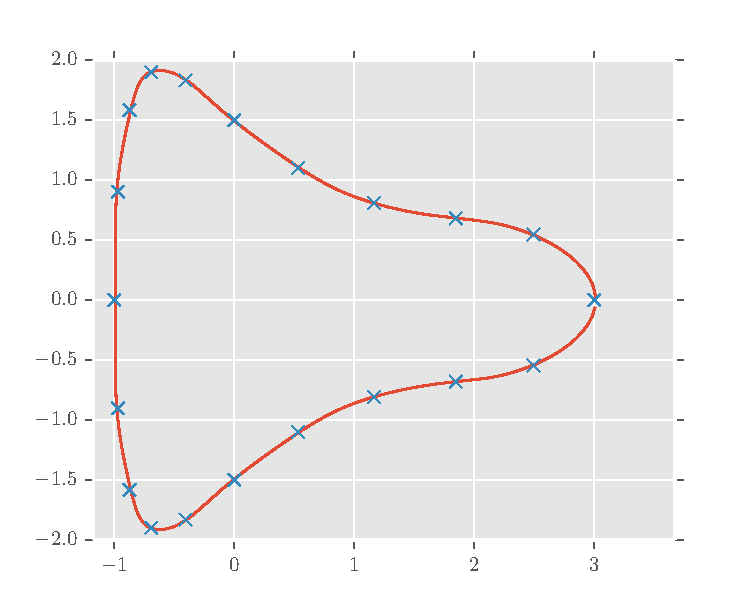
\includegraphics[keepaspectratio]{blob_shape.pdf}
  \end{center}
  \vspace{-.2in} % corrects bad spacing
  \caption{\label{fig:blob-shape} Example shape.}
\end{figure}

The equations for the initial shape are the following ($T_i$ is the i\textsuperscript{th} Chebyshev polynomial)

\begin{align*}
  x_1(0, s) = \cos(s) \paren{2 T_0\paren{\frac{s-\pi}{\pi}} + T_2\paren{\frac{s-\pi}{\pi}}}\\
  x_2(0, s) = \sin(s) \paren{2 T_0\paren{\frac{s-\pi}{\pi}} + T_4(\paren{\frac{s-\pi}{\pi}})}
\end{align*}

The method used to represent the shape numerically will be explained in Section \ref{sec:numerical-modeling}, but first we will take a moment to explain the various erosion processes that we will model in this section.

\subsection*{Continuous Erosion Processes}

All the processes that we will look at in this section, will move all points on the surface in a direction normal to the surface at each point, where the surface normal is defined as follows

\[
  \hat{n}(\vec{x}(s)) = (-\dot{\vec{x}}_2(s), \dot{\vec{x}}_1(s))
\]

In contrast to modeling erosion as a discrete process, as was done in the previous section, we will now model it with the following differential equation

\begin{equation}
  \frac{\partial \vec{x}(t, s)}{\partial t} = g(\vec{x}(t, s)) \; \hat{n}(t, s) \label{eq:erosion-diff-eq}
\end{equation}

for some function $g(\vec{x}(s))$ that depends on the erosion process.

\subsubsection*{Smoothing Process}

One of the processes that we will look at is a soap bar being worn down by a person holding it in their hand, which we will call the \textit{Smoothing Process}. In this process, the corners of the surface will get worn down quickest, because they are the first parts of the surface to come into contact with the person's hand. Technically the furthest protruding bumps will be worn down quickest, but to simplify the problem, we consider every point of the surface to wear down at a rate proportional to the curvature at the point. We will use a signed curvature $\kappa$, so that a bump will have positive curvature, and an indentation will have negative curvature. 

\[
  \kappa(\vec{x}(s)) = \frac{\dot{\vec{x}}(s) \times \ddot{\vec{x}}(s)}{\norm{\dot{\vec{x}}(s)}^3}
\]

$g(\vec{x}(s))$ for this model is the following

\begin{equation}
  g(\vec{x}(s)) = \tan^{-1}(\beta \, (\kappa(\vec{x}(s)) - \alpha)) + \frac{\pi}{2}
\end{equation}

For our simulations we chose $\alpha = 1, \; \beta = 5$ so that $g(\vec{x}(s)) \le 3$ ($\kappa(\vec{x}(0, s)) \in [-2, 2]$). This restriction is not based on the physics of the problem, and was chosen purely for the aesthetic look of the resulting simulation.

\begin{figure}[H]
    \begin{center}
      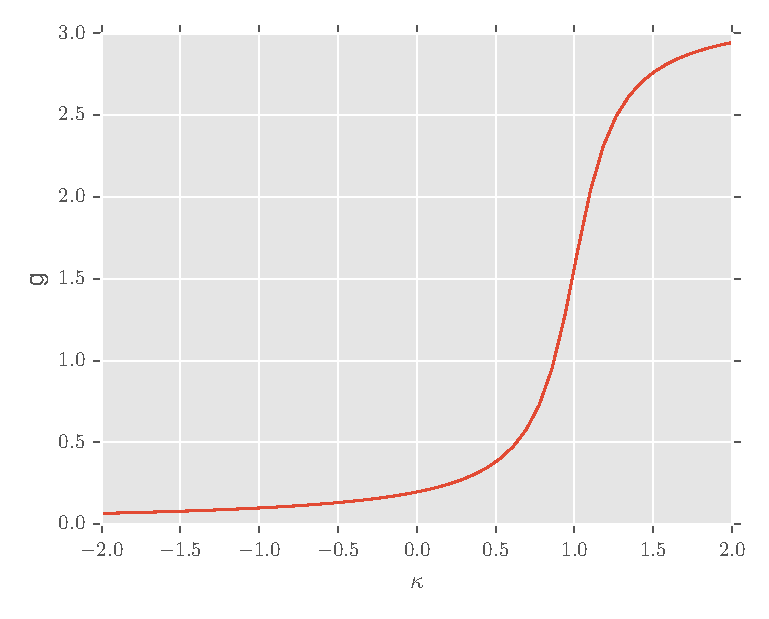
\includegraphics[keepaspectratio]{g_1.pdf}
    \end{center}
  \vspace{-.2in} % corrects bad spacing
  \caption{\label{fig:g-1} Plot of $g(\kappa)$ for \textit{Smoothing Process}.}
\end{figure}

\subsubsection*{Bottom Recession Process}

Our second process is an object sitting in a bath of acid, which we will call our \textit{Bottom Recession Process}. In this process, given a time $t_1$, the lowest points (smallest values of $\vec{x}_2(t_1, 0)$) on the surface will erode quickest. $g(\vec{x}(s))$ for this model is the following

\begin{gather}
  x_{2, min}(t) = \min(x_2(s)) \notag\\
  f(s) = \frac{1}{\alpha \, (x_2(s) - x_{2, min}(t)) + \beta} - \gamma \notag\\
  g(s) = \begin{cases}
    f(s) \qquad &\text{for} \quad f(s) > 0\\
    0 \qquad &\text{otherwise}
  \end{cases}
\end{gather}

For our simulations we chose $\alpha = 10, \; \beta = \gamma = 0.1$ so that $g(\vec{x}(s)) \approx 1$ for $x_2(s) \approx x_{2,min}$.

\begin{figure}[H]
    \begin{center}
      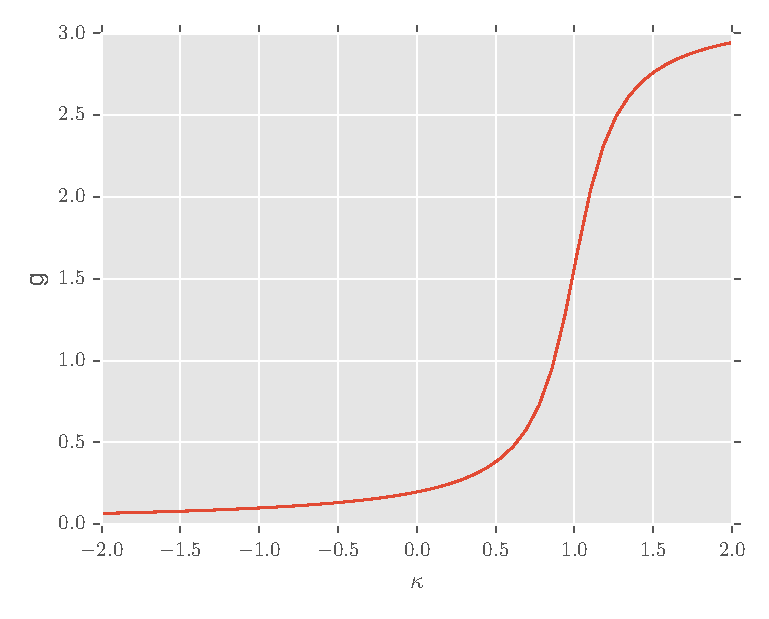
\includegraphics[keepaspectratio]{g_1.pdf}
    \end{center}
  \vspace{-.2in} % corrects bad spacing
  \caption{\label{fig:g-2} Plot of $g(y)$ for \textit{Bottom Recession Process}.}
\end{figure}


\subsection*{Numerical Modeling}\label{sec:numerical-modeling}

We chose to model the parametric surface functions with Discrete Fourier series. This is because spectral methods will maintain the smoothness of the surface much better than a local approximation of the surface using finite differences which only acts locally at points. The DFT and surface derivatives can be calculated quickly using the Fast Fourier Transform (refer to Appendix \ref{sec:dft} for more details).

To integrate Equation \ref{eq:erosion-diff-eq}, we sample the surface at parameter values $s_n = 2 \pi \, \frac{n}{N} \; , \; n = 0, \dotsc, N-1$, which gives us a matrix of initial evaluation points

\begin{align*} 
  \boldsymbol{x}_0 = \begin{bmatrix}
    x_1(0, s_1)& x_2(0, s_1)\\
    \vdots& \vdots\\
    x_1(0, s_N)& x_2(0, s_N)\\ 
  \end{bmatrix}
\end{align*}

Forward time integration of Equation \ref{eq:erosion-diff-eq} can then be implemented with standard ODE time stepping integration methods. In this paper, we used SciPy's {\tt odeint} method for integrating Equation \ref{eq:erosion-diff-eq}.

\subsection*{Point Collision Problems}

Unfortunately, the simplicity gained from modeling the surface with a Fourier series is soon lost when we start time stepping. As can be seen in Figure \ref{fig:remove-lowest-blob-bad}, the surface forms loops as time is increased (a physical impossibility).

\begin{figure}[H]
    \begin{center}
      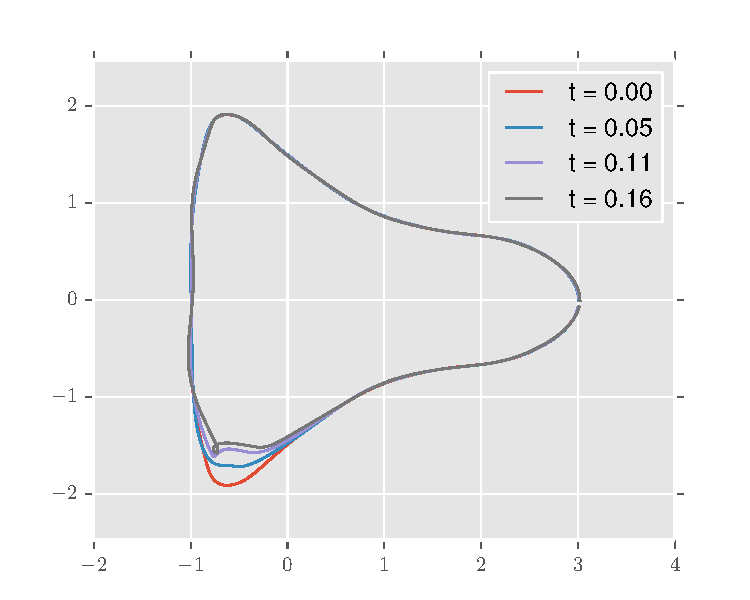
\includegraphics[keepaspectratio]{remove_lowest_blob_bad.pdf}
    \end{center}
  \vspace{-.2in} % corrects bad spacing
  \caption{\label{fig:remove-lowest-blob-bad}}
\end{figure}

To investigate why this occurs, we will show a zoomed in portion of the same figure, with the evaluation points shown. 

\begin{figure}[H]
    \begin{center}
      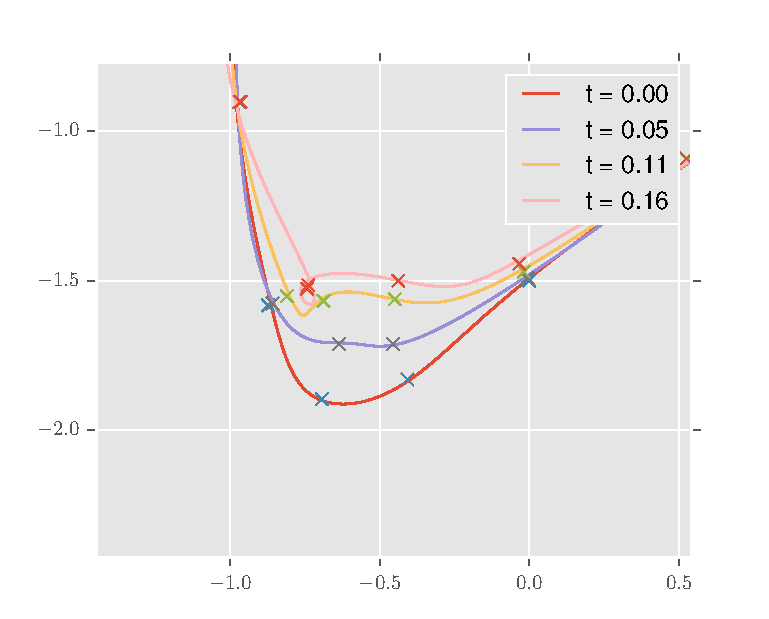
\includegraphics[keepaspectratio]{remove_lowest_blob_bad_zoom.pdf}
    \end{center}
  \vspace{-.2in} % corrects bad spacing
  \caption{\label{fig:remove-lowest-blog-bad-zoom}}
\end{figure}

Looking closely, it can be seen that areas of high curvature form when evaluation points get close to each other, and this eventually leads to surface looping. Our guess is that this occurs because we are using discrete time stepping, so there are errors in the approximation of the shape's change with time. This is fine when the evaluation points are far from each other, but when they get close to each other, the errors become significant and affect the direction of the surface unit normal vectors. The folding causes unit normal vectors of nearby points to point at each other and which subsequently causes the points to cross over each other.

\subsection*{Redistributing Points}

A seemingly obvious way to fix this problem would be to interpolate and find a new set of evaluation points that are evenly spaced along the surface. This wouldn't be too difficult of a task, since we can integrate and interpolate via the FFT. Unfortunately, if we pick points on the surface at arbitrary values of $s$, we lose spectral accuracy, because our new points will be sampled at different parameter values $\tilde{s} \ne s$, but the Discrete Fourier transform assumes that the points are sampled at $s$. 


The DFT is still assuming the function is sampled at

\[ \boldsymbol{s}_n = 2 \pi \, \frac{n}{N} \; , \; \text{for} \; n = 0, \dotsc, N-1 \]  

When we redistribute, we are sampling at new parameter values $\boldsymbol{\tilde{s}} \ne \boldsymbol{s}$. In the continuous sense, this redistribution is defined by a parameter transformation

\[ 
  \tilde{s}(s) = h(s) \; s.t. \; \norm{\frac{\partial \vec{x}(s)}{\partial \tilde{s}(s)}} = constant
\]

Our shape function becomes

\[ \tilde{x}(s) = (x \circ h)(s) \]

There is absolutely no guarentee that the Fourier series of this composite function will decay at a reasonable rate, so the DFT with resolution N could poorly capture the surface shape. The method is not withough hope, since the technique of parameter transformation is utilized extensively in spectral methods such as the transformation $h(s) = \cos(s)$ used with Chebyshev spectral methods to cluster evaluation points near the endpoints of the domain. We just need to find a way to generate a parameter transformation, $h(s)$ such that that $(x \circ h)(s)$ has a rapidly decaying Fourier series.

\subsection*{Continuous Redistribution}

If we look at $\vec{x}(t, s)$ at some time $t = t_1$, then we can .

\begin{align}
  \frac{\partial \vec{x}_{r}(t_1, s, t')}{\partial t'}& = a_t(t_1, s, t') \frac{\dot{\vec{x}}_r(t_1, s, t')}{\norm{\dot{\vec{x}}_r(t_1, s, t')}} \; , \quad \vec{x}_r(t_1, s, 0) = \vec{x}(t_1, s)  \notag \\
  &= \frac{\ddot{\vec{x}}_r(t_1, s, t') \boldsymbol{\cdot} \dot{\vec{x}}_r(t_1, s, t')}{\norm{\ddot{\vec{x}}_r(t_1, s, t')} \; \norm{\dot{\vec{x}}_r(t_1, s, t')}} \; \frac{\dot{\vec{x}}_r(t_1, s, t')}{\norm{\dot{\vec{x}}_r(t_1, s, t')}} \label{eq:redist-diff-eq}
\end{align}

Now, since $\vec{x}(t_1, s)$ is infinitely differentiable, $\vec{x}_r(t_1, s, t')$ is infinitely differentiable for all $t'$. 

Now, 

Physically $\dot{\vec{x}}_r(t_1, s, t')$ is the surface tangent vector, and $\ddot{\vec{x}}_r(t_1, s, t')$ is the rate of change of this surface tangent vector with respect to $s$. The reasoning behind \ref{eq:redist-diff-eq} is that $\norm{\dot{\vec{x}}_r(t, s)}$ is inversely proportional to the density of points on the surface at $s$; we want to shift points away from denser areas, which means moving them in the direction of larger $\norm{\dot{\vec{x}}_r(t_1, s, t')}$, which is precisely the projection of $\ddot{\vec{x}}(t_1, s, t')$ onto the surface tangent vector. 

To simplify the numerical computation, we combine \ref{eq:erosion-diff-eq} and \ref{eq:redist-diff-eq} to get a single ODE

\begin{equation}
  \frac{\partial (\vec{x}(t, s))}{\partial t} = g(t, s) \; \bhat{n}(t, s) + a_t(t, s, 0) \; \frac{\dot{\vec{x}}(t_1, s)}{\norm{\dot{\vec{x}}(t_1, s)}}
\end{equation}

As can be seen in Figure \ref{fig:remove-points-blob-good}, this dramatically improves our algorithm.

\begin{figure}[H]
    \begin{center}
      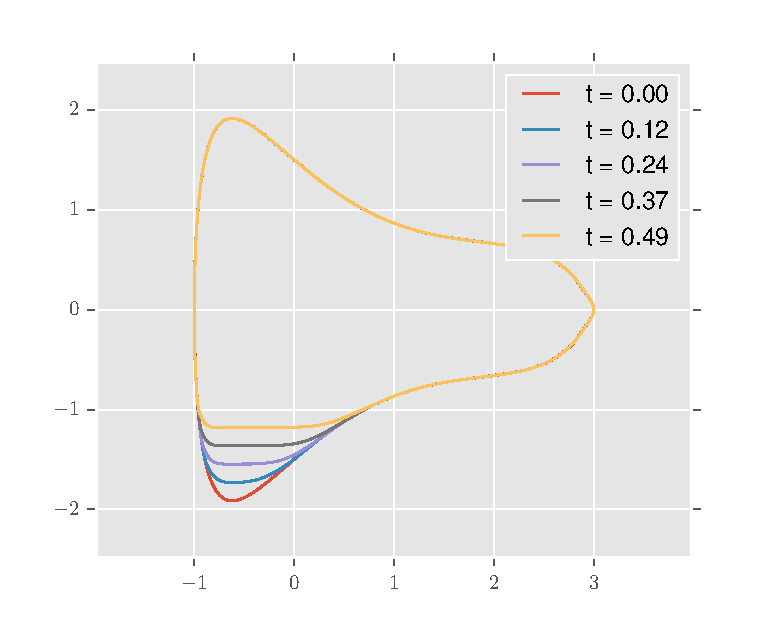
\includegraphics[keepaspectratio]{remove_points_blob_good.pdf}
    \end{center}
  \vspace{-.2in} % corrects bad spacing
  \caption{\label{fig:remove-points-blob-good}\textit{Bottom recession process} simulation with point redistribution.}
\end{figure}

If we plot the evaluation points (Figure \ref{fig:remove-points-blob-good-points}), it can be seen that the points nicely redistribute themselves as time increases to stay evenly spaced on the surface.

\begin{figure}[H]
    \begin{center}
      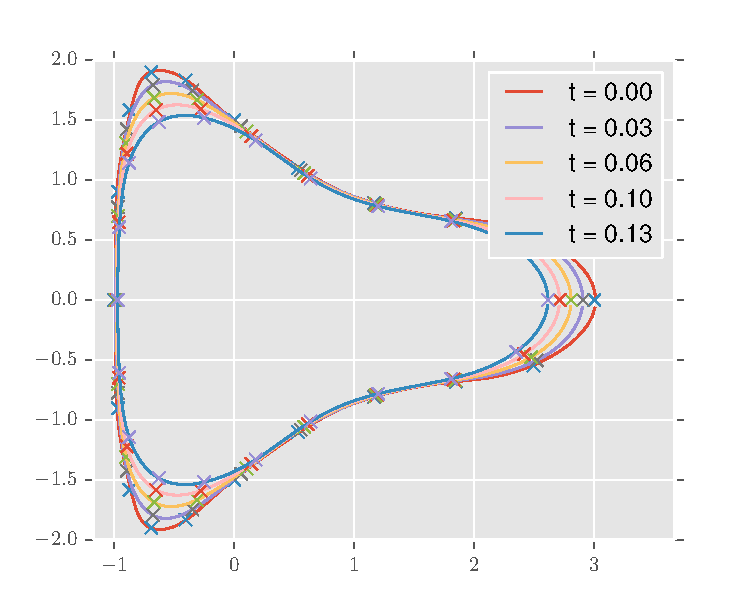
\includegraphics[keepaspectratio]{remove_points_blob_good_points.pdf}
    \end{center}
  \vspace{-.2in} % corrects bad spacing
  \caption{\label{fig:remove-points-blob-good-points}\textit{Smoothing process} simulation with evaluation points shown.}
\end{figure}

\subsection*{Higher dimensions}

A next logical step would be to generalize the algorithm to a 3-dimensional object. In that case, the surface would be 2-dimensional rather than 1-dimensional, so we woud need two parameters $s_1, s_2$. Much of the algorithm would be similar in 

\[
  \vec{n}(t, s_1, s_2) = \frac{\partial \vec{x}(t, s_1, s_2)}{\partial s_1} \times \frac{\partial \vec{x}(t, s_1, s_2)}{\partial s_2} 
\]

Curvature $\kappa$ would generalize to mean curvature $H$

\begin{align*}
  H(t, s_1, s_2)& = \frac{\nabla \boldsymbol{\cdot} \vec{n}(t, s_1, s_2)}{2}\\
  &= \frac{1}{2} \paren{\frac{\partial \vec{n}_1(t, s_1, s_2)}{\partial s_1} + \frac{\partial \vec{n}_2(t, s_1, s_2)}{\partial s_2}}
\end{align*}

The 2-dimensional DFT would also be needed 

